\documentclass[12pt]{article}

\usepackage[utf8]{inputenc}
\usepackage[english]{babel}
\usepackage{csquotes}

\newcommand{\VERSION}{0.1}

\usepackage{xcolor}
\usepackage{listings, lstautogobble}

\usepackage{graphicx}
\usepackage{subcaption}
\graphicspath{{./}{../fig/}}

\usepackage{booktabs}
\setlength{\heavyrulewidth}{1.5pt}
\setlength{\abovetopsep}{4pt}

% \lstset{language=bash,
% 	keywordstyle=\color{black},
% 	basicstyle=\small\ttfamily,
% 	commentstyle=\ttfamily\itshape\color{gray},
% 	stringstyle=\ttfamily,
% 	showstringspaces=false,
% 	breaklines=true,
% 	frameround=ffff,
% 	frame=single,
% 	rulecolor=\color{black},
% 	autogobble=true
% }

\usepackage{hyperref}
\hypersetup{
	colorlinks=true,
	linktoc=all,
	linkcolor=blue,
	citecolor=blue
}

\begin{document}
	
	\title{citFinder-\VERSION \space User Guide}
	\author{Aaron Maurais}
	\date{16 December 2018}
	
	\maketitle
	\tableofcontents
	\newpage

	\section{citFinder program outline} % (fold)
	\label{sec:citfinder_program_outline}

	\texttt{citFinder} consists of 3 phases: \hyperref[sub:input]{Input}, \hyperref[sub:analysis]{Analysis}, and \hyperref[sub:output]{Output}.

	\subsection{Input} % (fold)
	\label{sub:input}

	\begin{enumerate}
		\item Read each peptide from \texttt{DTAFilter-files} into a data structure in memory.
		\item Get peptide modification parameters from existing \texttt{sequest.params} files.
	\end{enumerate}

	% subsection input (end)

	\subsection{Analysis} % (fold)
	\label{sub:analysis}
	
	\begin{enumerate}%[label=\alph]
		\item Calculate b, y and neutral loss ions for each peptide
		\begin{itemize}
			\item By default, only $M+1$ ions are considered.
			\item The range of charge states to be considered can be specified with the \texttt{-minMZ} and \texttt{-maxMZ} options
		\end{itemize}
		
		\item Load the corresponding \texttt{.ms2} file into a buffer in memory
		
		\item Find the location of the scan in the \texttt{.ms2} file buffer and parse it into a \texttt{ms2::Spectrum} object

		\item Search the \texttt{ms2::Spectrum} object for fragment ions within a user defined tolerance.
		\begin{itemize}
			\item The tolerance can be specified with the \texttt{--matchTolerance} option.  The default tolerance is $M \pm 0.25 Th$. 
			\item If multiple ions are found in the specified range, ties are broken by intensity, \textit{i.e.} the most intense ion is chosen.
			\item This behavior can be modified with the \texttt{--multipleMatchCompare} option.
			\item In cases where multiple fragments have the same predicted mass, all possible fragments are considered to be found if the ion is found in the \texttt{ms2::Spectrum}.
		\end{itemize}

		\item Classify the fragment ions which were found.
		\begin{itemize}
			\item Fragment ions are classified into 5 possible groups according to the decision tree in Figure \ref{fig:ionType_tree}.

			\begin{itemize}
				\item \textbf{frag}: Any fragment ion which was found.
				\item \textbf{ambFrag}: B or Y ion which does not span the citrulline residue.
				\item \textbf{detFrag}: B or Y ion spanning citrulline residue.
				\item \textbf{detNlFrag}: Neutral loss fragment spanning citrulline residue and not containing N or Q.
				\item \textbf{ambNlFrag}: loss fragment spanning citrulline residue containing N or Q.
				\item \textbf{artNlFrag}: Neutral loss fragment not spanning citrulline residue.

			\end{itemize}

		\end{itemize}

		\item Determine whether the peptide contains citrulline based off the decision tree in Figure \ref{fig:containsCit_tree}.  

	\end{enumerate}

	\begin{figure}[h!]
			\centering
			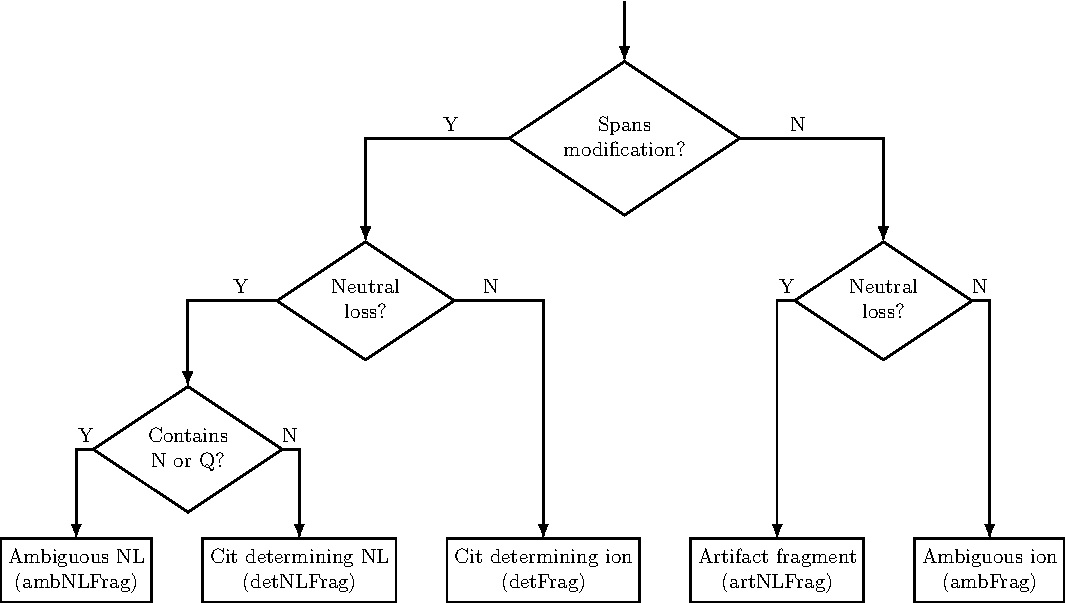
\includegraphics[width=\textwidth]{ionType_decision_tree.pdf}
			\caption{Decision tree for classifying fragment ion type}
			\label{fig:ionType_tree}
		\end{figure}

	\begin{figure}[h!]
		\centering
		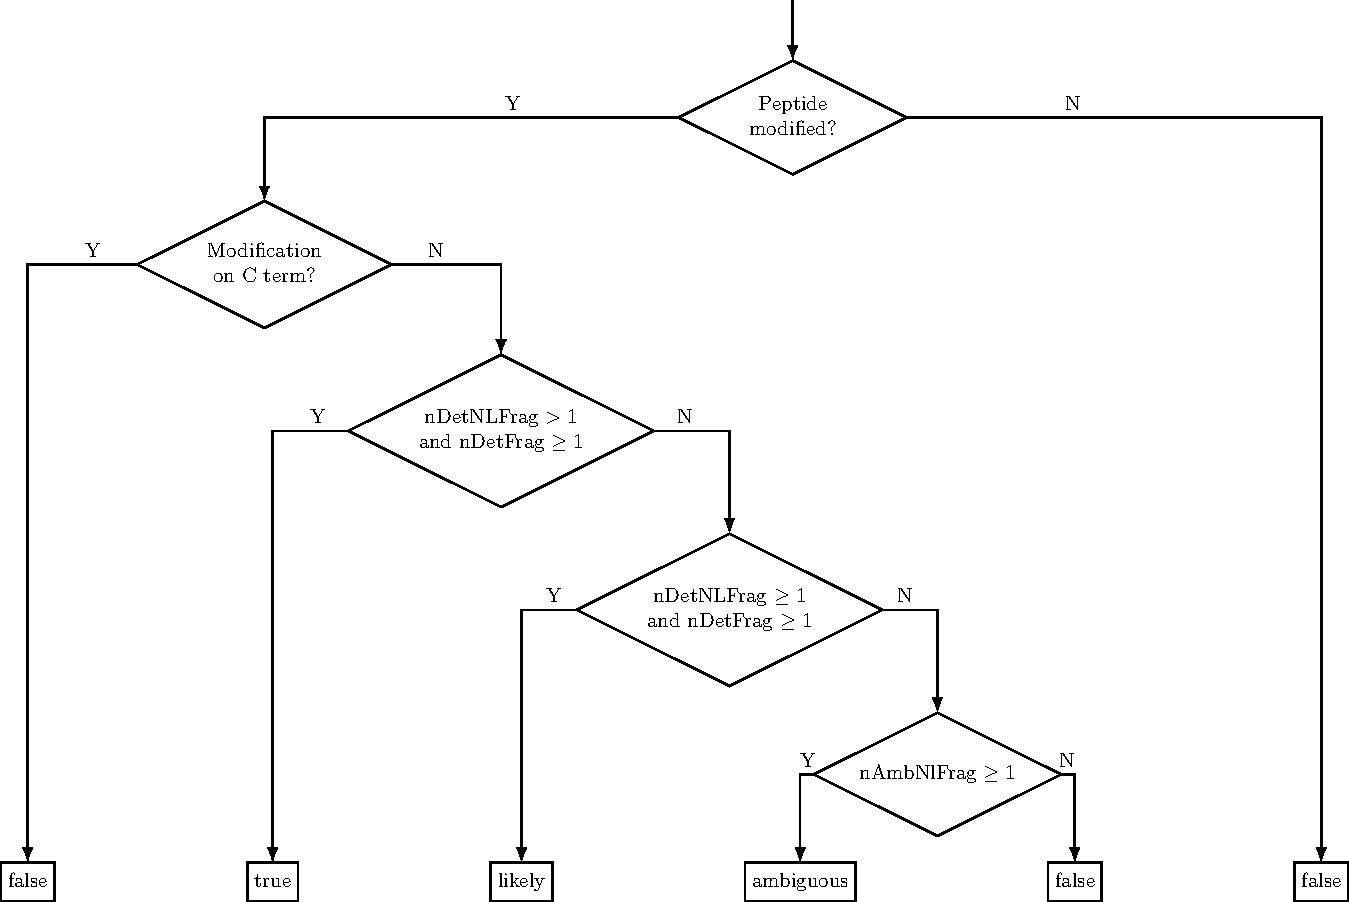
\includegraphics[width=\textwidth]{containsCit_decision_tree.pdf}
		\caption{Decision tree for determining whether a peptide contains citrulline.}
		\label{fig:containsCit_tree}
	\end{figure}

	% subsection analysis (end)

	\subsection{Output} % (fold)
	\label{sub:output}

	\begin{itemize}
		\item \texttt{peptide\_cit\_stats.tsv}
		\begin{itemize}
			\item Excel file with a line for each peptide, and columns for sequence, scan number, parent file, whether the peptide contains citrulline (output of decision tree in figure \ref{fig:containsCit_tree}) and numbers and types of ion classifications from decision tree in \ref{fig:ionType_tree}.  
		\end{itemize}

		\item If the \texttt{--printSpectra} option is specified, a \texttt{.spectra} file is generated which can be used to automatically generate a labeled ms2 from a peptide sequence.
		\begin{itemize}
			\item Example ms2s are shown in figure \ref{fig:ms2s}.
		\end{itemize}
	\end{itemize}

	\begin{figure}
		\centering
		\begin{subfigure}[b]{1\textwidth}
			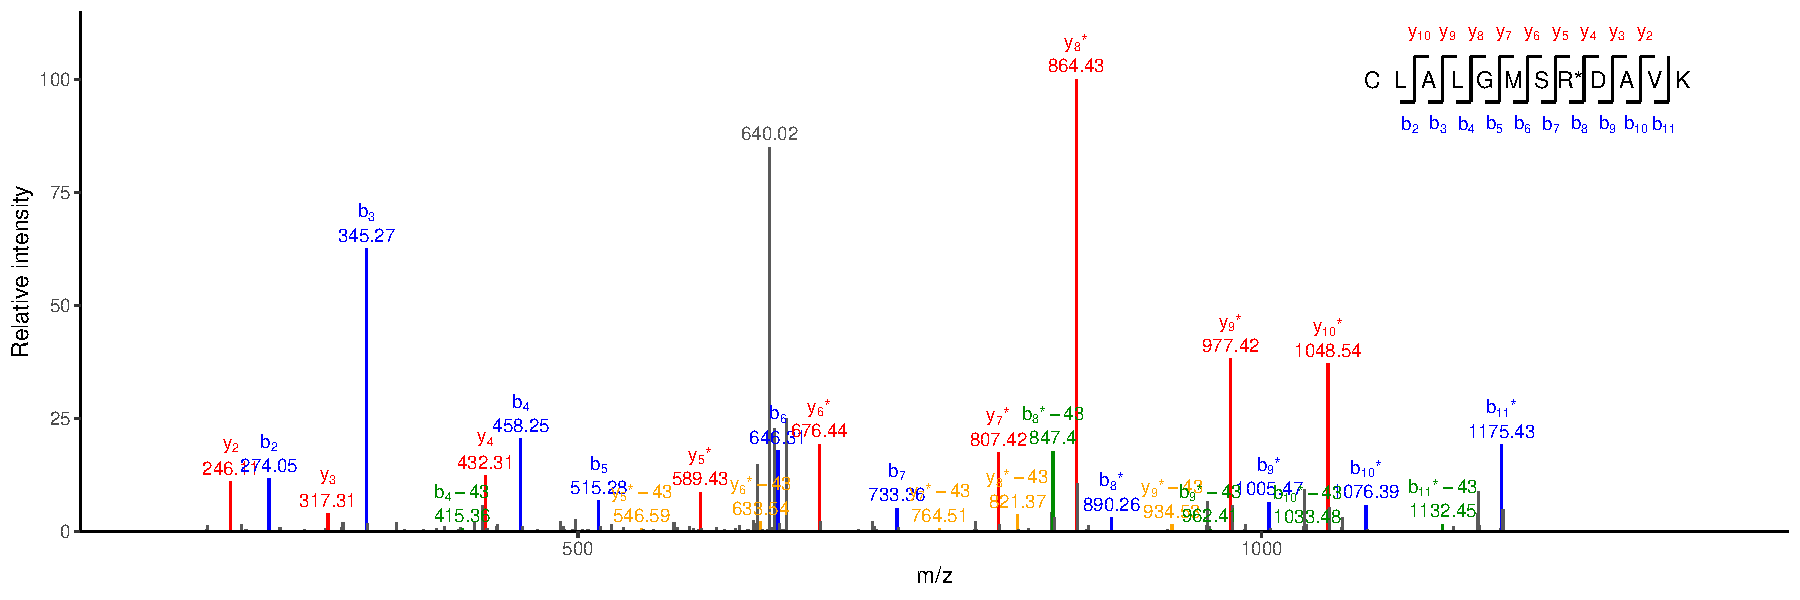
\includegraphics[width=\textwidth]{ror_pad_CLALGMSrDAVK_8469_2_nl.pdf}
			\caption{A good ms2}
			\label{sfig:good_ms2}
		\end{subfigure}

		\begin{subfigure}[b]{1\textwidth}
			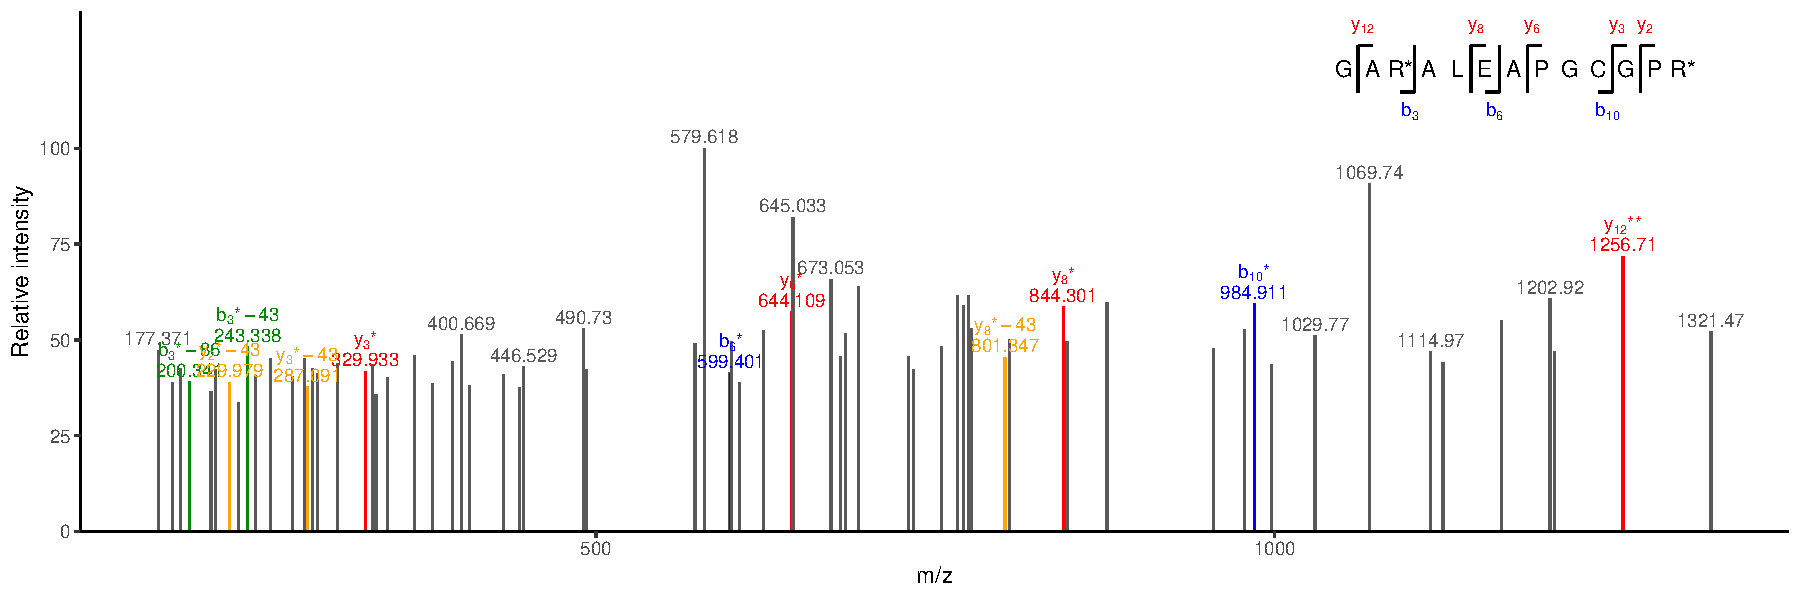
\includegraphics[width=\textwidth]{gat_pad_hr_GARALEAPGCGPR_11060_3.pdf}
			\caption{A bad ms2}
			\label{sfig:bad_ms2}
		\end{subfigure}

		\caption{Example labeled ms2s}
		\label{fig:ms2s}
	\end{figure}
	
	% subsection output (end)
	
	% section citfinder_program_outline (end)

	\section{TODO} % (fold)
	\label{sec:todo}

	\begin{enumerate}

		\item Figure out how to compile the program on \texttt{pleiades}. 
		\begin{itemize}
			\item This should be trivial, I just have to take the time to do it.
		\end{itemize}

		\item Write comprehensive documentation.
		\begin{itemize}
			\item I'd like to get the documentation to at least the point that the program is easy for you to use.
			%\item Also should be trivial.
		\end{itemize}

		\item Figure out how to classify fragment ions in peptides with multiple modified residues.
		\begin{itemize}
			\item Right now the fragments are classified according to the decision tree in Figure \ref{fig:containsCit_tree} for each citrulline modification, \textit{i.e.} a fragment will end up with two distinct classifications for each each citrulline modification.  
			\item There is currently no way to determine which modification the classification is referring to in the output file.
			\item I'd like your input on this. Is the way things are classified good enough for your use case, or would you rather be able to tell which individual citrulline modification was confirmed without manually looking at the ms2 your self?
			\item Again this is only a problem in cases where there are multiple citrulline residues on a peptide.
		\end{itemize}		

	\end{enumerate}

	% section todo (end)

\end{document}